\section{Existing solutions}
The customer wanted us to find out what kind of prototype device to develop connecting a social network and Arduino
into a tangible interface for the user. We did some research on the internet about similar and related products.  It is 
important to specify that our task was not to create another prototype, but create a  developer API that would ease 
future development of new protoypes connecting Arduino and any type of social network. The relevancy of these 
existing products for us was to confirm that it was possible to connect the user with Facebook in a tangible way using
 an Arduino. We also looked into social networks other than Facebook like Twitter or LinkedIn. Facebook is definitely the 
most popular social network out there, but it uses a proprietary API that is not compatible with the other social 
networks or open API implementations. We have included our most interesting ideas below, although we presented
many more to the customer:

\newpage

\subsection{LikeLight}
The customer initially showed us the prototype of a Facebook like indicator that would glow when some content the
user posted on Facebook was liked by someone. It was realized with an Arduino board inside a giant Lego hand. 
(Figure \ref{fig:prestudies-likehand})

\begin{figure}[h!]
\centering 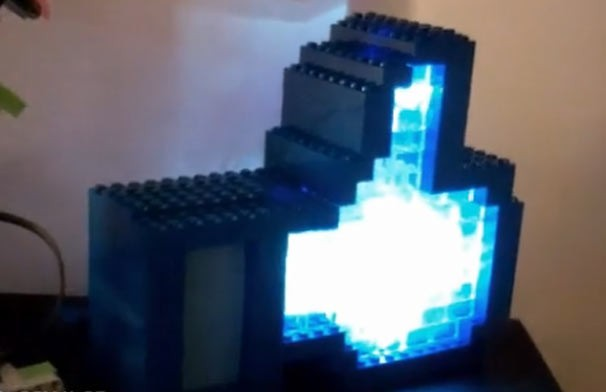
\includegraphics[scale=0.85]{img/prestudies-likehand} \caption{LikeLight from Red Pepper Labs}

\label{fig:prestudies-likehand}
\end{figure}

\newpage

\subsection{YepMailbox}
The YepMailbox (Figure \ref{fig:prestudies-YepMailbox}) was another concept of a tangible Arduino-powered prototype 
that would interact with the user Facebook wall. The mail flag would rise powered by a small servo motor and a printer 
would print out the new message.

\begin{figure}[h!]
\centering 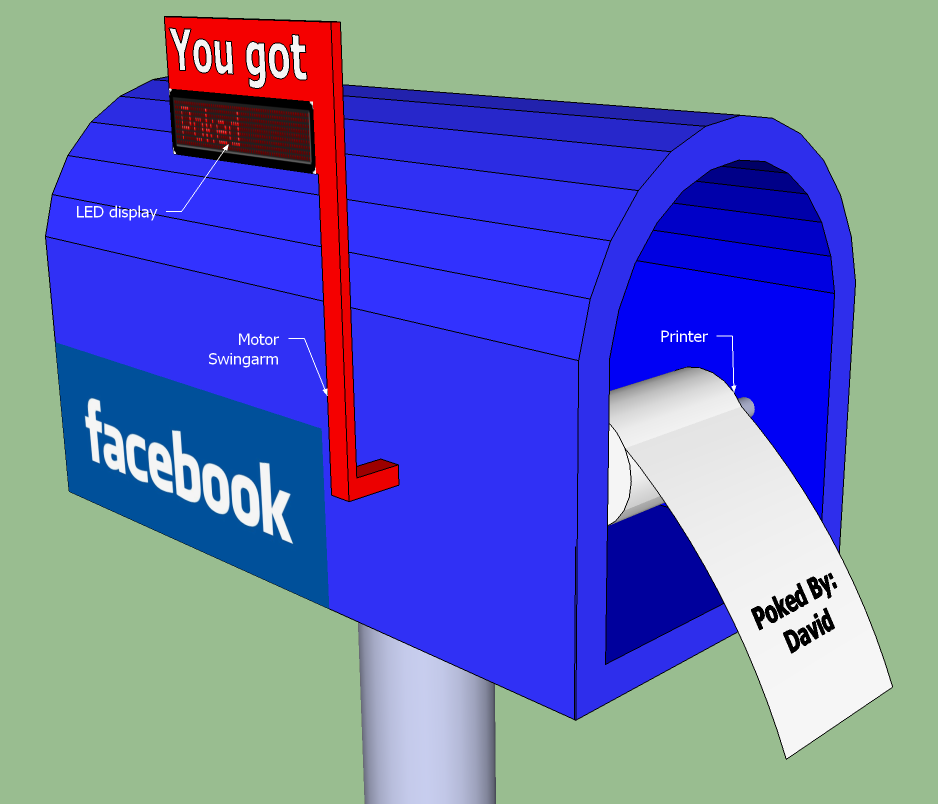
\includegraphics[scale=0.4]{img/prestudies-YepMailbox} \caption{Our concept idea of the YepMailbox}

\label{fig:prestudies-YepMailbox}
\end{figure}

\newpage

\subsection{Facebook Wall}
The "Facebook Wall" (Figure \ref{fig:prestudies-facebookwall}) is a be wall with two holes in it for people to put their faces in. 
The prototype would then make a picture and replace the wall with some image and add bodies to the two faces. The image 
would then be automatically uploaded and posted on Facebook.

\begin{figure}[h!]
\centering 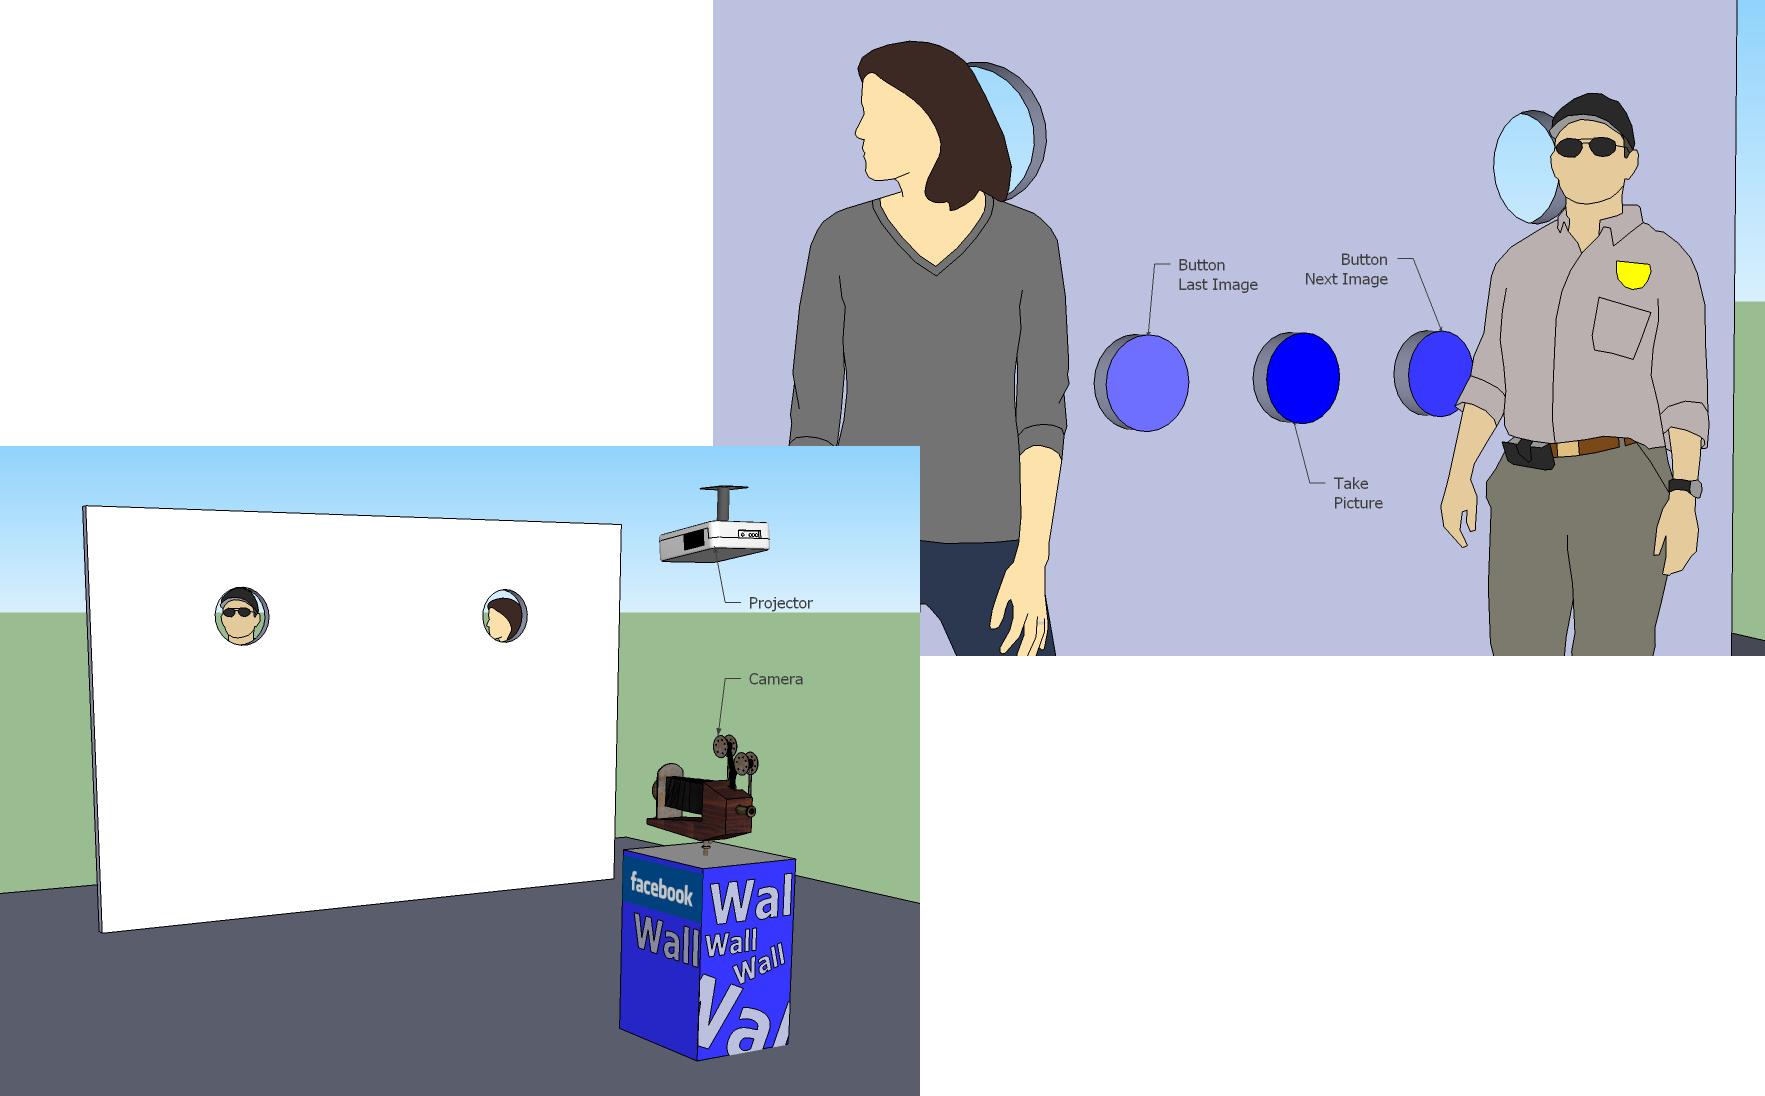
\includegraphics[scale=0.22]{img/prestudies-facebookwall} \caption{Our concept idea of the Facebook Wall}

\label{fig:prestudies-facebookwall}
\end{figure}

\newpage

\subsection{T-shirt}
The t-shirt (Figure \ref{fig:prestudies-tshirt})  has integrated electronic circuits powered by the Arduino Lilypad.
The Lilypad is an Arduino board designed especially to be wore.
It is connected wirelessly to the internet through an Android phone and downloads status updates from a social
networks such as Facebook. The content fetched is then displayed through one of the electronic devices, such as LED lamps,
LED screen, sound module or even a vibration modules.

\begin{figure}[h!]
\centering 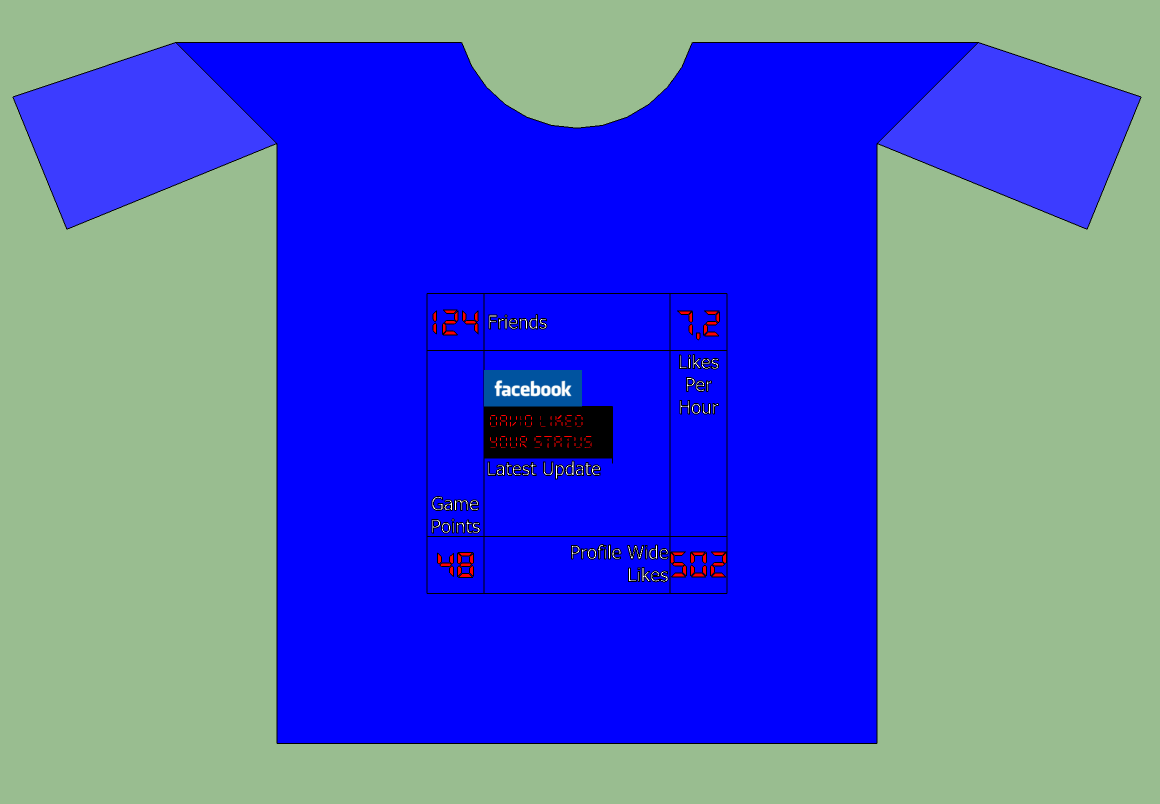
\includegraphics[scale=0.35]{img/prestudies-tshirt} \caption{Our first concept idea of the T-shirt prototype}

\label{fig:prestudies-tshirt}
\end{figure}

\subsection{Conclusion}
Ultimately we presented our various ideas and concepts to the customer and let him decide on what he would
like the group to work on. As a prototype he would like to see a T-Shirt connected to one or more social media
that will give the user updates on any changes or updates from social networks such as Facebook or Twitter.
This prototype would prove that our library can connect any social network (Twitter, Facebook, etc.) with any
tangible Arduino interface (LED, buzzer, sound, buttons, etc.). The customer requested one or two additional
smaller prototypes in addition to the T-Shirt to prove that our API works on any prototype device and is not
specific to the T-Shirt.
